\documentclass{beamer}
\usepackage{lmodern}
\usepackage{tikz}

\begin{document}

\title{SIAM-IMA Etymo workshop - institution extraction}
\author{Jonathan Deakin}
\date{\today}

\begin{frame}
  \maketitle
\end{frame}

\begin{frame}{Introduction}
  \begin{overlayarea}{\textwidth}{\textheight}
    \begin{itemize}
      \item<1-> Papers can be associated with an institution/s
      \item<2-> We may be interested in following a particular instituion:
      \item<3->[]
      \begin{center}
        \emph{What is Google doing?}
      \end{center}
      \item<4-> How do we extract the institution/s of a paper?
    \end{itemize}


  \end{overlayarea}
\end{frame}


\begin{frame}{What we have}
  \onslide<2->{\begin{tikzpicture}
    \node[anchor=south west,inner sep=0] at (0,0) {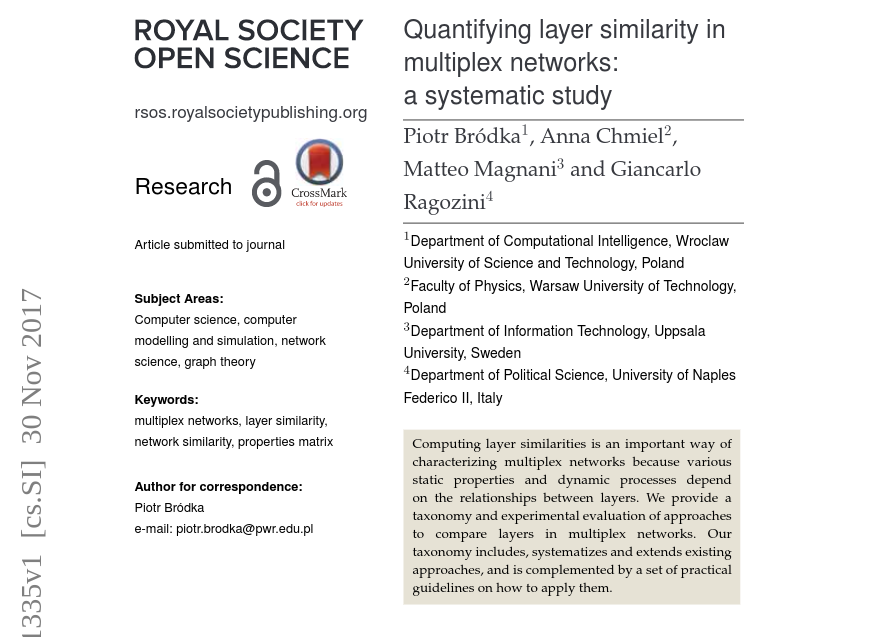
\includegraphics[width=\columnwidth]{first_page_example.png}};
    \draw<3->[red,thick,rounded corners] (4.9,4.55) rectangle (9.2,5.1);
    \draw<4->[red,thick,rounded corners] (4.9,3.98) rectangle (9.2,4.5);
    \draw<5->[red,thick,rounded corners] (4.9,3.45) rectangle (9.2,3.93);
    \draw<6->[red,thick,rounded corners] (4.9,2.8) rectangle (9.2,3.4);
  \end{tikzpicture}}
\end{frame}


\begingroup
\scriptsize
\begin{frame}{Actually what we have}

  rsos.royalsocietypublishing.org

  Research

  Article submitted to journal

  Subject Areas:
  Computer science, computer
  modelling and simulation, network
  science, graph theory

  Keywords:
  multiplex networks, layer similarity,
  network similarity, properties matrix

  Author for correspondence:
  Piotr Bródka
  e-mail: piotr.brodka@pwr.edu.pl

  7
  1
  0
  2



  v
  o
  N
  0
  3





  ]
  I
  S
  .
  s
  c
  [



  1
  v
  5
  3
  3
  1
  1

  .

  1
  1
  7
  1
  :
  v
  i
  X
  r
  a

  Quantifying layer similarity in
  multiplex networks:
  a systematic study
  Piotr Bródka1, Anna Chmiel2,
  Matteo Magnani3 and Giancarlo
  Ragozini4

  \only<1>{1Department of Computational Intelligence, Wroclaw
  University of Science and Technology, Poland
  2Faculty of Physics, Warsaw University of Technology,
  Poland
  3Department of Information Technology, Uppsala
  University, Sweden
  4Department of Political Science, University of Naples
  Federico II, Italy}

  \only<2->{{\color{red} 1Department of Computational Intelligence, Wroclaw
  University of Science and Technology, Poland
  2Faculty of Physics, Warsaw University of Technology,
  Poland
  3Department of Information Technology, Uppsala
  University, Sweden
  4Department of Political Science, University of Naples
  Federico II, Italy}}

  Computing layer similarities is an important way of
  characterizing multiplex networks because various
  static properties and dynamic processes depend
  on the relationships between layers. We provide a
  taxonomy and experimental evaluation of approaches
  to compare layers in multiplex networks. Our
  taxonomy includes, systematizes and extends existing
  approaches, and is complemented by a set of practical
  guidelines on how to apply them.

\end{frame}
\endgroup

\begin{frame}{Introduction}
  \begin{center}
    Insert IPython notebook here
  \end{center}
\end{frame}

\begin{frame}{Parting words}
  \begin{center}
    \begin{itemize}
      \item<1->[] Make it work,
      \item<2->[] Make it better,
      \item<3->[] Make it best
    \end{itemize}
  \end{center}
\end{frame}

\end{document}
